\documentclass[11pt,a4paper]{article}

% These are extra packages that you might need for writing the equations:
\usepackage{amsmath}
\usepackage{amsfonts}
\usepackage{amssymb}
\usepackage{booktabs}
\usepackage{hyperref}
\usepackage{listings}
\usepackage{xcolor}
\lstset {language=C++,
		 basicstyle=\ttfamily,
         keywordstyle=\color{blue}\ttfamily,
         stringstyle=\color{red}\ttfamily,
         commentstyle=\color{purple}\ttfamily,
         morecomment=[l][\color{magenta}]{\#},
       	 basicstyle=\tiny}

% You need the following package in order to include figures in your report:
\usepackage{graphicx}

% With this package you can set the size of the margins manually:
\usepackage[left=2cm,right=2cm,top=2cm,bottom=2cm]{geometry}


\begin{document}

% Enter the exercise number, your name and date here:
\noindent\parbox{\linewidth}{
 \parbox{.25\linewidth}{ \large HPCSE I, Exercise 03 }\hfill
 \parbox{.5\linewidth}{\begin{center} \large Beat Hubmann \end{center}}\hfill
 \parbox{.2\linewidth}{\begin{flushright} \large Oct 19, 2018 \end{flushright}}
}
\noindent\rule{\linewidth}{2pt}

\section{Question 1}

\subsection{Task a)}

The program was implemented as instructed and is attached to this submission.

\subsection{Task b)}
The results of running the compiled program on Euler and my own machine (a 2018 Macbook Pro) are plotted in figures~\ref{fig:1}~and~\ref{fig:2}. at the marks seen in the random task, but they are much less pronounced: While we're able to read from cache lines, reading the increasingly large arrays makes memory access a bottle neck.


\begin{figure}[ht]
\begin{center}
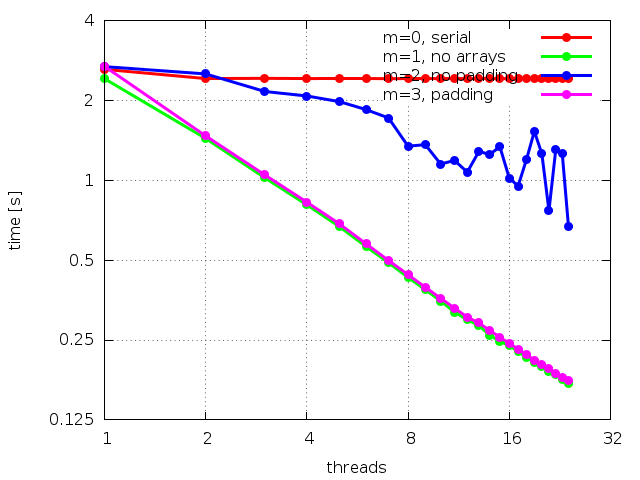
\includegraphics[scale=0.5]{results.png} 
\end{center}
\caption{blub Euler compute cluster.}
\label{fig:1}
\end{figure}

\begin{figure}[ht]
\begin{center}
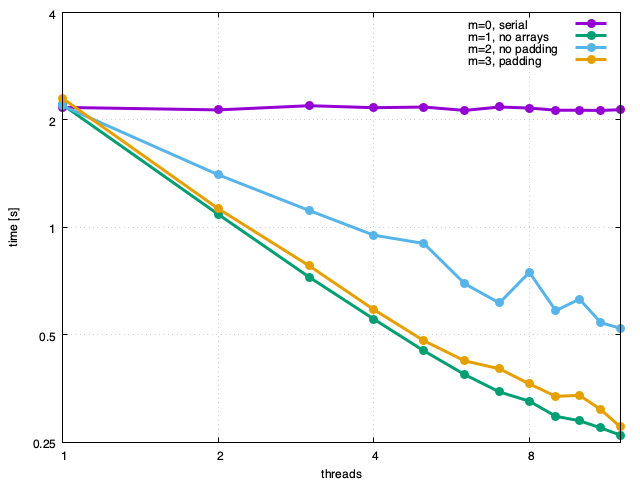
\includegraphics[scale=0.5]{results_mbp.png} 
\end{center}
\caption{blub 2018 Macbook Pro cluster.}
\label{fig:2}
\end{figure}



\section{Question 2}

There is a problem with the global variable \texttt{pos} in the \texttt{if} statement starting on line 13: In order to write to the array \texttt{good\_members}, the value of \texttt{pos}
must be read in line 14. This read is not protected from race conditions with the atomic write on line 17. As \texttt{\#pragma omp atomic} cannot be extended to several statements, a possible (but still ugly)
solution would be to replace the \texttt{for} loop block from lines 12 to 19 with snippet~\ref{lst:1}.

\begin{lstlisting}[float, caption='Blub', label={lst:1}]
    #pragma omp parallel for
    for (int i= 0; i < N; i++)
    {
        if (is_good(i)) // No change until here
        {
            int thread_pos{0}; // Define thread specific position variable
            #pragma omp critical // This block replaces the #pragma omp atomic section
            {
                thread_pos= pos; // Protected read
                pos++; // Protected write
            }
            good_members[thread_pos]= i; // Use thread specific variable
        }
    }
\end{lstlisting}




%\begin{itemize}
%\item{Cache is empty (i.e. cold)}
%\item{"Memory transfer" implies transfer from random access memory (DRAM) to cache (typically L3 cache)}
%\end{itemize}
%
%\subsubsection{DAXPY}
%
%\begin{equation}
%y = \alpha x + y \quad \alpha \in \mathbb{R}; x, y \in \mathbb{R}^{n}
%\end{equation}
%
%According to table~\ref{tab:daxpy}, a DAXPY operation on $x, y \in \mathbb{R}^{n}$ requires $2n$ FLOPS and $3n$ memory accesses. By definition, \textbf{D}AXPY is a double precision operation and thus each involved element has a size of 8 bytes. The resulting total operational intensity is $I(n) = \frac{2n \: \text{FLOPS}}{3n \cdot 8 \: \text{bytes}} = \frac{1}{12} \: \text{ops/byte}$ and hence $\mathcal{O}(1)$.
%
%\begin{table}[ht]
%\centering
%\begin{tabular}{@{\extracolsep{4pt}}lcccc}
%\toprule
%{}  & \multicolumn{2}{c}{FLOPS} & \multicolumn{2}{c}{memory accesses}\\
%\cmidrule{2-3}
%\cmidrule{4-5}
%$i = 1,2, \ldots, n$ & multiply & add & read & write \\
%\midrule
%$n \: \text{times\ldots} $  & 1    & 1   & 2   & 1 \\
%\bottomrule
%\end{tabular}
%\caption{DAXPY operations per element $i \in \{1, 2, \ldots, n\}$}\label{tab:daxpy}
%\end{table}
%
%\subsubsection{SGEMV}
%
%\begin{equation}
%y = Ax + y \quad x, y \in \mathbb{R}^{n}; A \in \mathbb{R}^{n \times n}
%\end{equation}
%
%According to table~\ref{tab:sgemv}, a SGEMV operation on $x, y \in \mathbb{R}^{n}$ requires $2n^2 + n$ FLOPS and $2n^2 + 2n$ memory accesses. To make things easier we focus on the asymptotic bound and only consider the second-order terms. By definition, \textbf{S}GEMV is a single precision operation and thus each involved element has a size of 4 bytes. The resulting total asymptotic operational intensity is $I(n) = \frac{2n^2\: \text{FLOPS}}{2n^2\cdot 4 \: \text{bytes}} = \frac{1}{4} \: \text{ops/byte}$ and hence $\mathcal{O}(1)$.
%
%\begin{table}[ht]
%\centering
%\begin{tabular}{@{\extracolsep{4pt}}lcccc}
%\toprule
%{}  & \multicolumn{2}{c}{FLOPS} & \multicolumn{2}{c}{memory accesses}\\
%\cmidrule{2-3}
%\cmidrule{4-5}
%$i = 1,2, \ldots, n$ & multiply & add   & read   & write \\
%\midrule
%$n \: \text{times\ldots} $                    & $n$      & $n+1$ & $2n+1$ & 1 \\
%\bottomrule
%\end{tabular}
%\caption{SGEMV operations per element $i \in \{1, 2, \ldots, n\}$}\label{tab:sgemv}
%\end{table}
%
%
%\subsubsection{DGEMM}
%
%\begin{equation}
%C = AB + C \quad A,B,C \in \mathbb{R}^{n \times n}
%\end{equation}
%
%Based on the hint given in the task description, we assume that $n$ and thus the matrices $A, B, C$ are small enough to fit in the cache concurrently and do not require multiple reads during a single DGEMM operation. According to table~\ref{tab:dgemm}, a DGEMM operation on $B, C \in \mathbb{R}^{n \times n}$ requires $2n^3 + n^2$ FLOPS and only $4n^2$ memory accesses because of the above assumption about $n$ versus cache size. As for SGMEV above, we focus on the higher order terms for the following calculations. By definition, \textbf{D}GEMM is a double precision operation and thus each involved element has a size of 8 bytes. The resulting total asymptotic operational intensity is $I(n) = \frac{2n^3\: \text{FLOPS}}{4n^2\cdot 8 \: \text{bytes}} = \frac{n}{16} \: \text{ops/byte}$ and hence $\mathcal{O}(n)$.
%
%\begin{table}[ht]
%\centering
%\begin{tabular}{@{\extracolsep{4pt}}lcccc}
%\toprule
%{}  & \multicolumn{2}{c}{FLOPS} & \multicolumn{2}{c}{memory accesses}\\
%\cmidrule{2-3}
%\cmidrule{4-5}
%$i,j = 1,2, \ldots, n$ & multiply & add   & read   & write \\
%\midrule
%$n\cdot n \: \text{times\ldots} $                    & $n$      & $n+1$ & $3$ & 1 \\
%\bottomrule
%\end{tabular}
%\caption{DGEMM operations per element $i, j \in \{1, 2, \ldots, n\}$}\label{tab:dgemm}
%\end{table}
%
%
%\subsection{Task b)}
%
%\begin{equation}
%u_{i}^{n+1} = u_{i}^{n} + \frac{\Delta t \alpha}{\Delta x^2}(u_{i-1}^{n} - 2u_{i}^{n} + u_{i+1}^{n})
%\label{eqn:1d_diffusion}
%\end{equation}
%
%Based on equation~(\ref{eqn:1d_diffusion}) and considering that $\frac{\Delta t \alpha}{\Delta x^2}$ is a fixed value which can be precalculated and stored, there are 3 additions and 2 multiplications for a total of 5 FLOPS per grid point. As for DGEMM in the previous task, we now must make assumptions about the problem size versus the cache size (the cache size being a potential bottleneck): It would be most realistic but also most cumbersome for our calculations to assume that some part of the problem fits in a cache of limited but realistic size and that we have to deal with a mix of compulsory and capacity cache misses. At the extreme ends of the cache size-vs-problem size scale we could take up either the assumption of an infinite cache and thus only one read and one write operation per grid point or the assumption of zero cache with a worst case maximum of four reads and one write per grid point. Assuming we are dealing with double precision data (8 bytes per element), we can thus make the following estimations: $I(N)_{\text{max}} = \frac{5\: \text{FLOPS}}{2\cdot8 \: \text{bytes}}=\frac{5}{16}\: \text{ops/byte}$ and $I(N)_{\text{min}} = \frac{5\: \text{FLOPS}}{5\cdot8 \: \text{bytes}}=\frac{1}{8}\: \text{ops/byte}$ with the realistic asymptotic operational intensity bounded as in equation~(\ref{eqn:task3b}).
%\begin{equation}
%0.125  \: \text{ops/byte} \leq I(N) \leq 0.3125  \: \text{ops/byte}
%\label{eqn:task3b}
%\end{equation}



%\begin{thebibliography}{99}
%
%\bibitem{nasa}
%	NASA,
%	\emph{Haswell Processors},
%	online (\url{https://www.nas.nasa.gov/hecc/support/kb/haswell-processors_492.html}),
%	accessed 30-Sep-2018.
%
%\bibitem{intel}
%	Intel Corporation,
%	\emph{Intel Xeon Processor E5-2680 v3 Product Specifications},
%	online (\url{https://ark.intel.com/products/81908/}),
%	accessed 30-Sep-2018.
%	
%\bibitem{euler}
%	ETH Zurich,
%	\emph{scientific computing wiki: Euler},
%	online (\url{https://scicomp.ethz.ch/wiki/Euler#Euler_II}),
%	accessed 30-Sep-2018.	
%
%\bibitem{kou}
%	Petros Koumoutsakos,
%	\emph{HPCSE I Lecture Notes},
%	online (\url{http://www.cse-lab.ethz.ch/wp-content/uploads/2018/09/HPCSE_I_1_Intro.pdf}),
%	accessed 30-Sep-2018.
%
%\end{thebibliography}
%

%\appendix
%\section{Question 4, task d)}\label{app}
%\lstinputlisting{ex01_q4_task_d.cpp}
\end{document}